\subsection{Introducción}
El problema trata sobre un un grupo de arqueólogos y caníbales que quieren cruzar un puente pero se encuentran con el problema de que solo disponen de una sola linterna para cruzarlo. Solo pueden cruzar como mucho dos personas y no pueden dejar que los caníbales sean mayoría en ningún momento pues estos últimos se los comerían. \\

Para ejemplificarlo mejor vamos a mostrar una imagen representando una posible instancia del problema:


%\begin{figure}
%	\centering
%	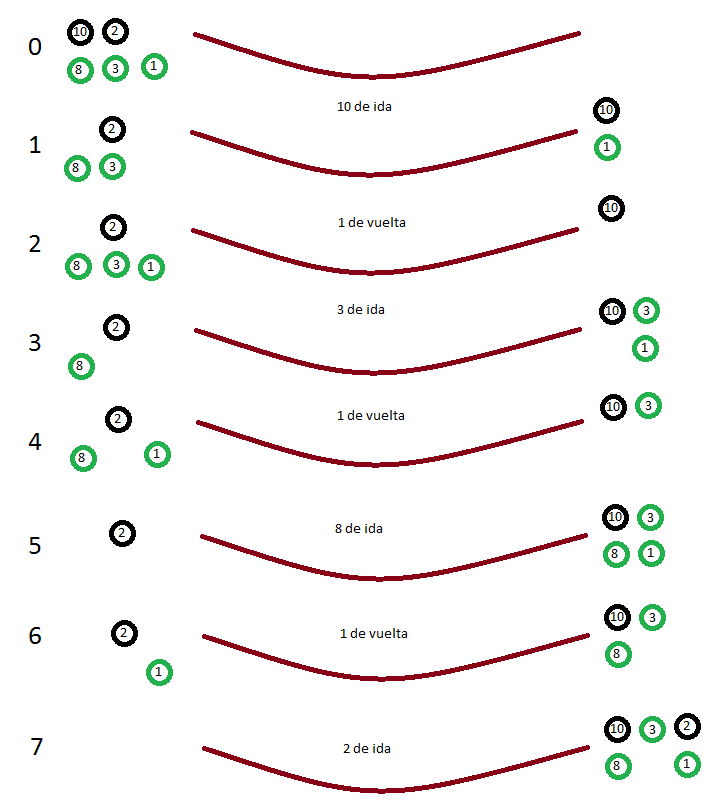
\includegraphics[width=1.5cm]{images/canibalesYArqueologos.png}
%	\caption{Ejemplo de posible instancia.}
%\end{figure}

\begin {figure} [H]
\begin {center}
 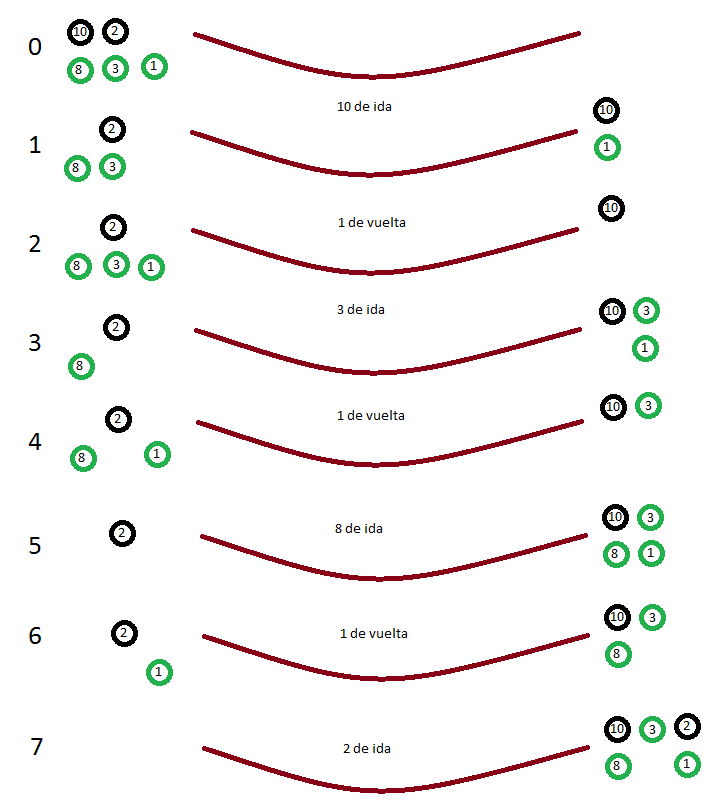
\includegraphics[width=0.8\textwidth,natwidth=610,natheight=642]{images/canibalesYArqueologos.png}
 \caption{Ejemplo de posible instancia.}
\end {center}
 \end{figure}

Dada esta situacion inicial, vamos a intentar ejemplificar como es el mecanismo para resolver esta instancia y asi explicar de que se trata el problema.

Tenemos 6 personas, 2 caníbales y 3 arqueólogos. Cada uno de estos tiene una velocidad asociada y sabemos que las personas pueden pasar de grupos de a dos o de a uno, si los que pasan son dos entonces la velocidad de cruzado es igual a la velocidad del más lento de los dos, además también hay que tener en cuenta que la linterna es una sola y por lo tanto tiene que volver para poder seguir cruzando. Otra cosa a tener en cuenta es que en ninguno de los dos lados del puente puede haber mas caníbales que arqueologos (pués se los comerían), en el único caso que puede llegar a pasar esto es cuando hay solo caníbales y ningún arqueólogo ya que no tendrían a quién comerse.

Siguiendo con el ejemplo, en el paso 1 vamos a intentar llevar un grupo de dos, con la persona mas rápida para aprovechar su velocidad a la hora de volver con la linterna. El tema de elegir con quien ir en cada paso es fundamental, ya que si se elige por ejemplo dos caníbales, obligatoriamente vamos a tener que traer dos arqueólogos y volver con un caníbal, ya que de otra forma los caníbales serían mayoría del otro lado del puente.

Seguimos entonces por llevar un caníbal y un arqueólogo. Notar que en ningún momento se deja mas caníbales que arqueólogos. Eso es algo a tener en cuenta. Es por eso que es necesario saber bien a quién vamos a ir pasando y quién es el que va a volver con la linterna.
En los siguientes pasos se va dando prioridad a que vuelva el de mayor velocidad ya que (metiéndonos también un poco en la resolución) de esta forma, aprovechamos que vuelve solo y es la persona que menos tarda en cruzar el puente.

\subsection{Resoluci\'on}
Para la resolución vamos permutando las instancias pero con la restricción del enunciado, que es sólo poder mandar una o dos personas desde donde esta la linterna hacia el otro lado, pasando la linterna también.\\
La instancia inicial es: todas las personas de un mismo lado y la linterna a la izquierda. \\
Usamos la técnica de backtracking, la instancia inicial sería la raíz, y vamos bajando a medida que permutamos. El primer problema que se presenta es cómo no repetir permutaciones en una misma rama para no entrar en una rama infinita, para ésto cada padre va agregando a su hijo al conjunto de instancias, y le pasas este conjunto en la recursión al hijo. Cuando el hijo vuelve de la recursión el padre lo saca del conjunto (por si la permutación se repite pero en otra rama o sub-rama a partir del padre).

\subsubsection{Justificaci\'on de la soluci\'on}

\textbf{Identificación de cada instancia de manera única}: 
Cada instancia consiste de: una lista de persona en la izquierda, una lista de personas en la derecha y si la linterna esta en la izquierda o en la derecha.
Además podemos identificar cada instancia sólo mirando la lista izquierda y dónde está la linterna (no es necesario además mirar la lista derecha ya que dado un grupo de personas iniciales y dos listas izquierdas iguales, las listas de la derecha deben ser iguales). 
\newline
\newline
Para identificar cada instancia de una forma numérica usamos la escritura en binario. Inicialmente a cada persona le asignamos una \emph{ID} distinta, empezando en $0$ e incrementándola en uno por cada persona.
\\
Luego, armamos un arreglo de $n + 1$ elementos, siendo $n$ la cantidad inicial de personas. En este arreglo vamos a poner en la posición $i$ un $1$ o un $0$ si la persona con \emph{ID} $i$ está en la izquierda o si está en la derecha, respectivamente. En la posición $n$ hacemos lo mismo pero para la linterna.
De esta manera nos queda la representación en binario de un número al que vamos a usar para identificar a cada instancia.
   \newline
   \newline
   \textbf{Estructura del backtracking}:
   Para entrar a la raíz del árbol, y a los demás nodos nos metemos con esta función, que se llama una vez:
\begin{verbatim}
Recursión(Lista izq, Lista vacia, int tiempoOptimo, int tiempoActual, bool linternaIzq, Conjunto instancias, Arreglo instancia_actual)
\end{verbatim}   
Donde:
\begin{itemize}
\item izq: Es la lista de personas que están en la izquierda, en el caso inicial están todas las personas con sus números primos ya asignados
\item der: Van a estar todos los que están en la derecha, en el caso inical está vacía.
\item tiempoOptimo: En esta  variable nos vamos guardando el tiempo óptimo, al principio vale cero, y mientras valga 0 no habremos llegado a ninguna solución aún (Si al volver de toda la recursión sigue siendo cero, es porque no se puedo encontrar ninguna solución al problema inicial)
\item tiempoActual: Nos vamos guardando el tiempo que vamos sumando a medida que pasamos personas al otro lado, inicialmente es 0.  
\item instancias: es un conjunto tipo árbol que vamos manteniendo a medida que bajamos por la rama. Es decir, el padre inserta el ID del hijo al que va a saltar la recursión, y lo borra cuando el hijo vuelve, para así poder bajar por otra rama de instancias. \\ Es necesario que el padre borre al hijo del conjunto cuando éste vuelve, ya que al bajar por otra rama está bien que se repitan instancias de otras sub-ramas, porque sería una solución distinta. 
\item instancia\_actual: es el arreglo que nos sirve para identificar la instancia de la que venimos y así actualizarla para pasársela a la siguiente llamada.
\end{itemize}

\textbf{Cada vez que entramos a un nodo tenemos:}
\begin{lstlisting}
    IF (No hay personas del lado izquierda) 
        return minimo(tiempo optimo, tiempo actual); 
        
    ELSE IF(tiempo actual > tiempo optimo) return tiempo optimo;
\end{lstlisting}
\begin{itemize}
\item Chequeamos si en esta instancia no tenemos personas en la izquierda, es decir llegamos a una solución. En es caso afirmativo devolvemos el mínimo entre el tiempo óptimo (el tiempo que tardó la mejor solución que tenemos hasta ahora) y el tiempo actual (tiempo que nos tomó llegar hasta esta instancia).
\item Si el tiempo actual es mayor que el tiempo óptimo quiere decir que las soluciones que encontremos a partir de este nodo van a ser peores de lo que ya tenemos. Por lo tanto no vale la pena seguir bajando por el árbol. 
\end{itemize}

\textbf{Armar la instancia "hijo"}:

\textbf{Estrategia 1}:
\begin{itemize}
\item Linterna derecha: La instancia siguiente la armamos mandando de a uno hacia la izquierda, cuando ya recorrimos la lista derecha de esa forma, empezamos a mandar de a uno hacia la izquierda.
\item Linterna izquierda: Idem que lo anterior pero de de izquierda a derecha.  

\end{itemize}

      \textbf{Estrategia 2}:
\begin{itemize}
\item Linterna derecha: La instancia siguiente la armamos mandando de a uno hacia la izquierda, cuando ya recorrimos la lista derecha de esa forma, empezamos a mandar de a dos hacia la izquierda.
\item Linterna izquierda: En este caso comenzamos a mandar de a dos, y luego mandamos de a uno. Esto lo hacemos porque en todas las soluciones que intentamos a mano, en ninguna había que mandar de a dos personas de izquierda a derecha, por lo tanto nos pareció pertinenter mandar así para poder llegar a una primera solución de manera mas rápida. \\ Sin embargo puede ser que en algún problema haya que mandar de a uno de izquierda a derecha, entonces también tenemos que intentar buscar esa posible solución.  

\end{itemize}
      \textbf{Estrategia 3}:
\begin{itemize}
\item Esta estrategia es igual a la anterior, salvo que cuando mandamos de a una persona no recorremos toda la lista de lo que podemos mandar, si no que mandamos al caníbal mas rápido y luego al arqueólogo mas rápido. 
Sea una solución no óptima $S$ y una instancia de el algoritmo para llegar a $S$ en la que mandamos a una persona $P$. Asumiendo que $P$ es arqueólogo entonces mandando a otro arqueólogo $P'$ llegamos a otra solución $S'$. En particular elegimos a $P'$ como al arqueólogo mas rápido de los que están del lado de la linterna.
 
Como $tiempo(P')$ $\leq$ $tiempo(P)$ entonces al pasarlo al otro lado en $S'$ sumamos menos tiempo que al pasar $P$ en $S$. 
En alguna instancia posterior puede que $P'$ vuelva con otra persona $T$, pero como $P'$ es mas rápido que $P$, entonces el tiempo de pasar a estos dos es: $max(tiempo(P'),$ $tiempo(T))$ $\leq$ $max(tiempo(P),$ $tiempo(T))$.

Por lo tanto el costo de $S'$ es mejor o igual que el costo de $S$, y así nos armamos una solución mejor.
\end{itemize}
En cada caso actualizamos el arreglo que identifica a la instancia actual poniendo un $0$ o un $1$ en la posición de la $ID$ de la persona que mandamos a la derecha o a la izquierda. Además en la última posición actualizamos si la linterna se va a la derecha o a la izquierda.
\newpage
\textbf{Pasar al siguiente nodo}:
Una vez armada la instancia siguiente, calculamos el tiempo máximo de la ó las personas que mandamos, para sumárselo al tiempo actual.
\begin{lstlisting}
    tiempo actual += tiempo max(personas que pasan)

    ID Instancia = Numero(arreglo instancia_actual) 				

    IF( Izquierda es valida & Derecha es valida & !Pertenece(ID Instancia, instancias){	
			
          Agregar(ID Instancia, instancias)
				
          tiempo optimo = Recursion( Izquierda, Derecha, tiempo optimo, tiempo actual, !linterna actual, instancias, arreglo instancia_actual);
				
          Borrar(ID Instancia, instancias)
    }
    tiempo actual-= tiempo max(personas que pasan);	
\end{lstlisting}

\begin{itemize}
\item Al principio sumamos al tiempo actual el máximo de las dos o una personas que tenemos para mandar.
\item \begin{verbatim}
ID Instancia = Numero(arreglo instancia_actual) 				
\end{verbatim}
Nos guardamos en $instID$ el valor numérico de la instancia, calculando en base diez el numero en binario representado en el arreglo de instancia actual.
\item \begin{verbatim}
IF( Izquierda es valida & Derecha es valida & !Pertenece(ID Instancia, instancias){	
\end{verbatim}
Chequeamos si nos quedó una instancia válida, o sea mas arqueólogos que caníbales o sólo caníbales, en cada lado. Y también si la instancia que armamos ya la repetimos mas arriba en la rama, fijandonos si está en el conjunto de instancias. \\ Como explicamos antes, repetir instancias en una misma rama no tendría sentido para la solución óptima e incluso tendríamos una rama infinita. 
\item \begin{verbatim}
          Agregar(ID Instancia, instancias)
				
          tiempo optimo = Recursion( Izquierda, Derecha, tiempo optimo, tiempo actual, !linterna actual, instancias, arreglo instancia_actual);
				
          Borrar(ID Instancia, instancias)
				
\end{verbatim}
Cómo la instancia es válida y no está repetida en la rama, entonces la agregamos al conjunto de instancias por las que ya pasamos.\\
Luego nos metemos en la recursión con lo que tenemos y al volver sacamos la instancia del conjunto de instancias de la rama, esto es para que no influya en otras ramas distintas o sub-ramas de este nodo. 
\item Por último arreglamos el tiempo actual restándole el tiempo que habíamos sumado de las personas que mandamos, para que siempre quede el tiempo actual del nodo actual. 
\end{itemize}

\textbf{Nota:} Cuando volvemos a la primer recursión original, nos fijamos si el tiempo optimo es $0$, en ese caso no llegamos a ninguna solución y devolvemos $-1$, si no, devolvemos el tiempoOptimo.

\subsection{Cota de Complejidad}
Puede estimarse una cota superior acotando groseramente una rama, y así obteniendo la altura del árbol. \\
Ya que lo único que hacemos es ir permutando las instancias a medida que bajamos por una rama, mirando toda la rama puedo tener todas las permutaciones posibles de la lista inicial junto con la linterna. Esta cantidad es la suma de combinatorios de ir tomando de a dos elementos, de a tres, etc. Todo esto multiplicado por $2$ por la linterna.
Entonces, siendo A la altura del árbol y $n$ la cantidad de personas: 
\[A = 2 * \sum_{i=1}^{n}\binom  {n} {i}\ = 2 * (\sum_{i=0}^{n}\binom  {n} {i}\ -1) = 2 * ((\sum_{i=0}^{n}\binom  {n} {i} *1^{n-i} * 1^{i})\ - 1) = 2 * ((1 + 1)^n\ - 1) = 2 * (2^n - 1)
\]
\\
Para obtener la cantidad de hojas, falta calcular la cantidad de hijos que tiene un nodo. Como vamos mandando de a una persona, y luego de a dos, es claro que cada nodo tiene $\binom{n}{1}$ $+$ $\binom{n}{2}$ $=$ $n + (n*(n-1))/2$ $=$ $((n^2 + n)/2)$ hijos. \\
Por lo tanto la cantidad de hojas es: $((n^2 + n)/2)^{A}$
\\
\\
El costo en cada nodo es: 
\begin{itemize}
\item $\mathcal{O}(3n)$ por clonar dos listas y el arreglo de la instancia.
\item $\mathcal{O}(n + n + log(n))$ por fijarse si una instancia es válida, sacar la ID de la instancia y fijarse en el conjunto de instancias si no es repetida.
\item $\mathcal{O}(2log(n))$ por agregar y borrar sobre el conjunto de instancias recorridas. 
\item En total la suma de todos estos costos es $\mathcal{O}(n)$
\end{itemize}
\textbf{Cota total}:
Por lo tanto la complejidad total es $\mathcal{O}(((n^2 + n)/2)^A) *\mathcal{O}(n)$ $=$ $\mathcal{O}((n^2)^A*n)$ $=$ $\mathcal{O}(n^{2A+1})$ % Open at top left 
\subsection{Experimentación}

\par Para realizar pruebas sobre el algoritmo implementado, dividimos los casos de entrada en 3 tipos:
\begin{itemize}
	\item \textbf{Iguales:} Todas las velocidades de las personas son iguales. Para realizar las pruebas las seteamos todas en 10, pero este valor es anecdótico, ya que no influye realmente en el rendimiento del programa.
	\item \textbf{Pocas Diferencias:} Las velocidades de las personas varían en un rango acotado. Nos pareció interesando testear casos donde la diferencia de velocidades no sea grande. Para las pruebas seteamos valores entre 10 y 20.
	\item \textbf{Algunas Diferencias:} Las velocidades de las personas varían en un rango mucho mayor al caso anterior, pero sigue siendo un rango acotado. Este caso es interesante para verificar las podas agregadas al algoritmo y como utiliza estas diferencias de velocidades para descartar casos. Para realizar las pruebas tomamos los valores 10 y 500 y los repartimos entre las personas.
	%\item \textbf{Uno Muy Diferente:} La velocidad de uno difiere mucho con la del resto de las personas. Este caso también es interesando de ver para verificar que las podas realmente sirvan. Para realizar las pruebas le asignamos a una persona el valor 500 y al resto el valor 10.
\end{itemize}

\par Para cada uno de los casos mecionados vamos a correr todas las combinaciones de personas diez veces cada caso. Mediremos el tiempo de ejecución y tomaremos la mediana de estos valores para evitar outliers y otros inconvenientes. Luego observaremos y analizaremos los resultados.

\begin {figure} [H]
\begin {center}
 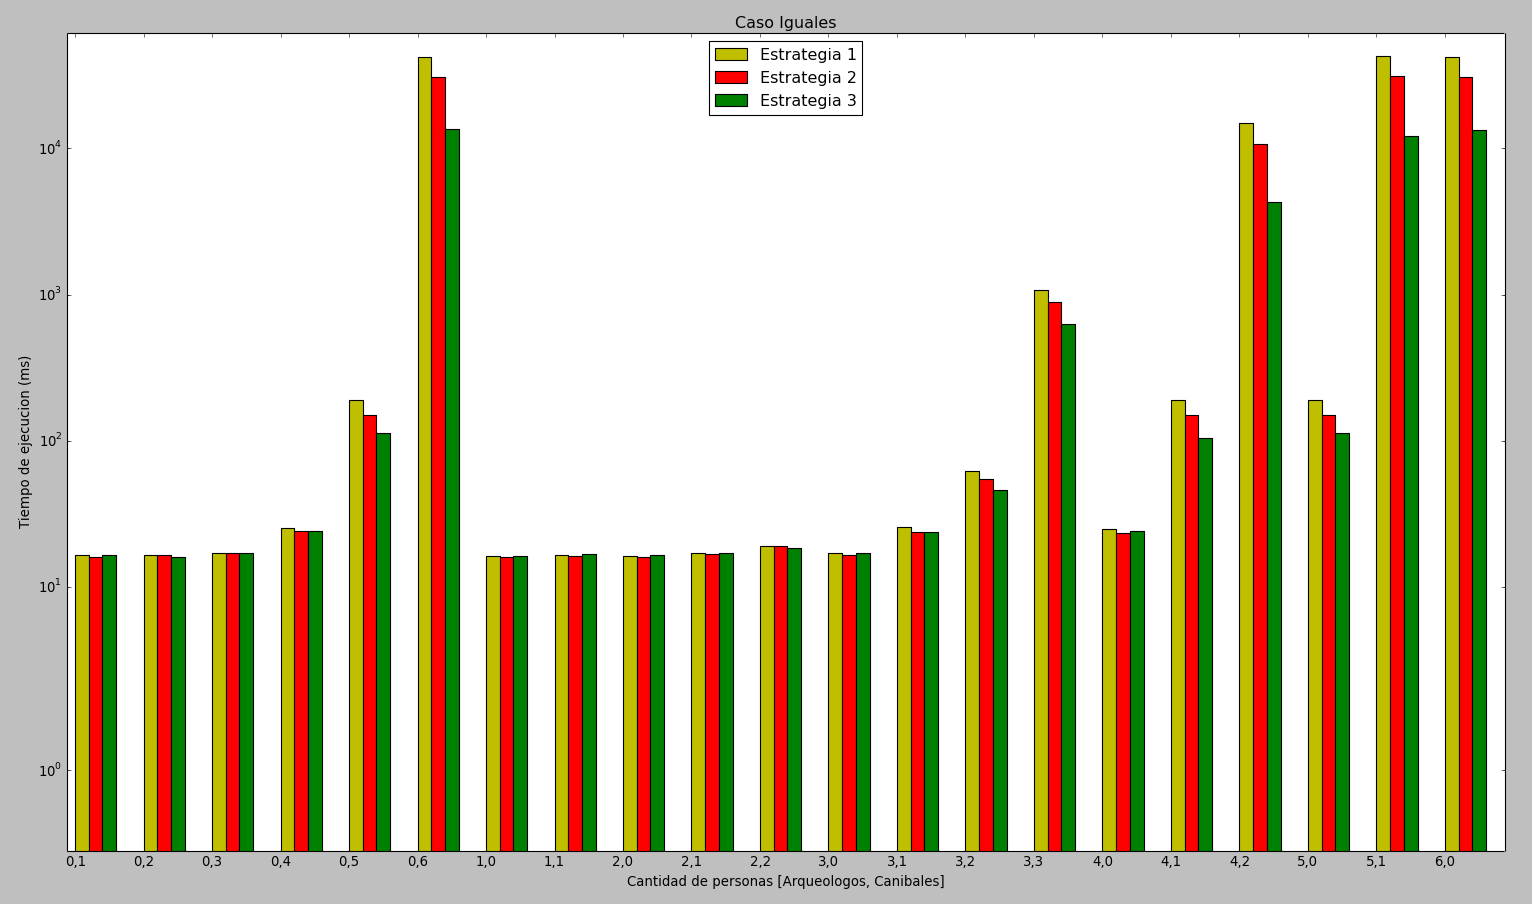
\includegraphics[width=1\textwidth,natwidth=610,natheight=642]{images/iguales.png}
 \caption{Caso donde todos tienen la misma velocidad.}
\end {center}
 \end{figure}
 \begin {figure} [H]
\begin {center}
 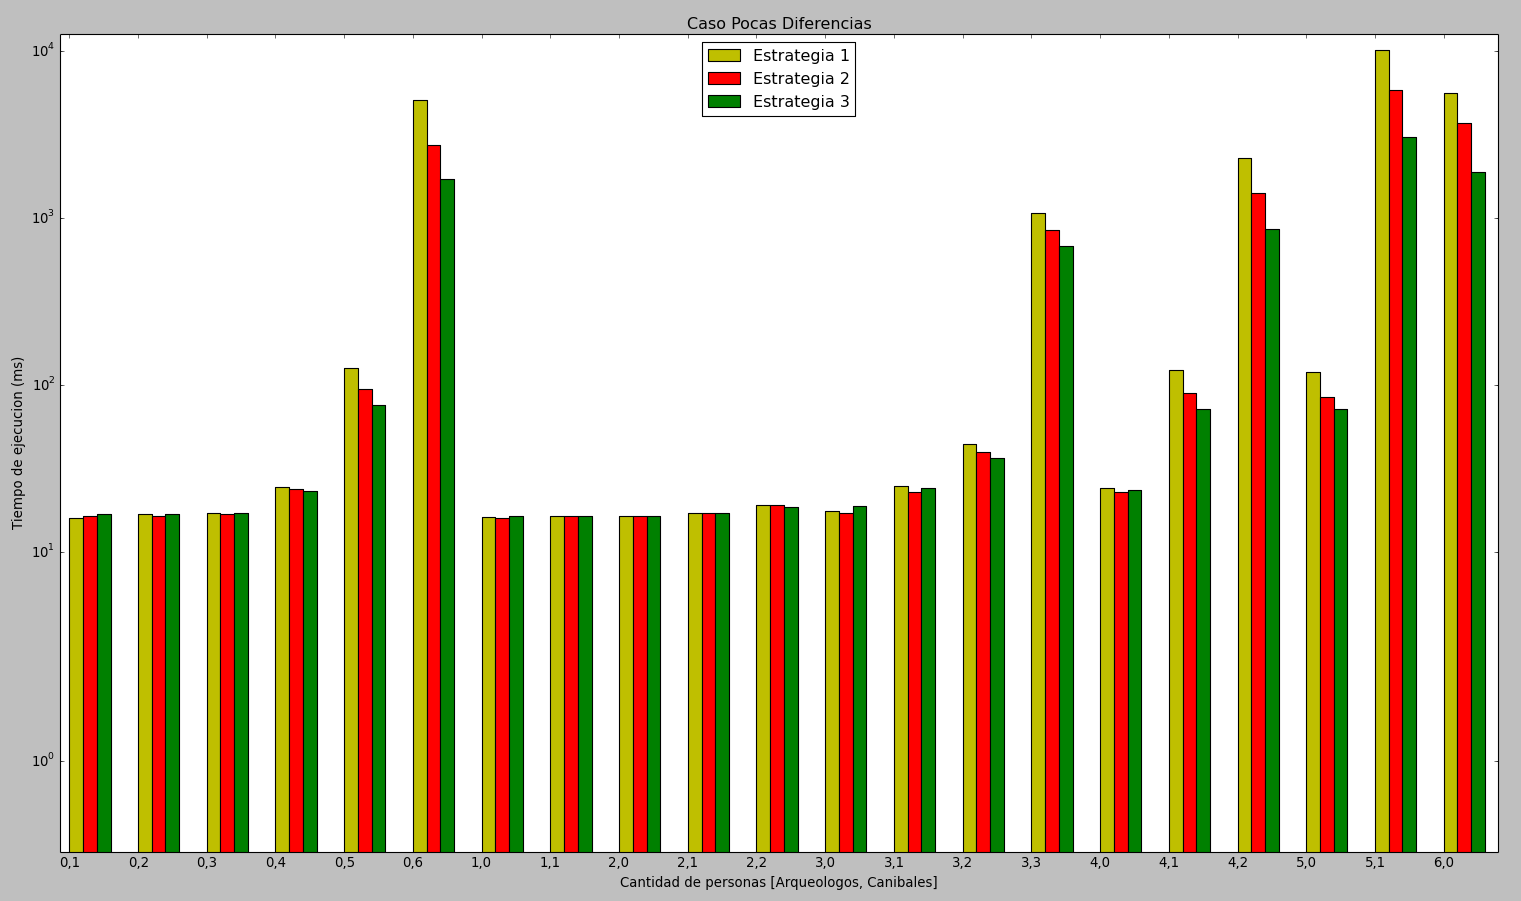
\includegraphics[width=1\textwidth,natwidth=610,natheight=642]{images/pocas_diferencias.png}
 \caption{Caso con velocidades que tienen poca diferencia entre ellas.}
\end {center}
 \end{figure}
 \begin {figure} [H]
\begin {center}
 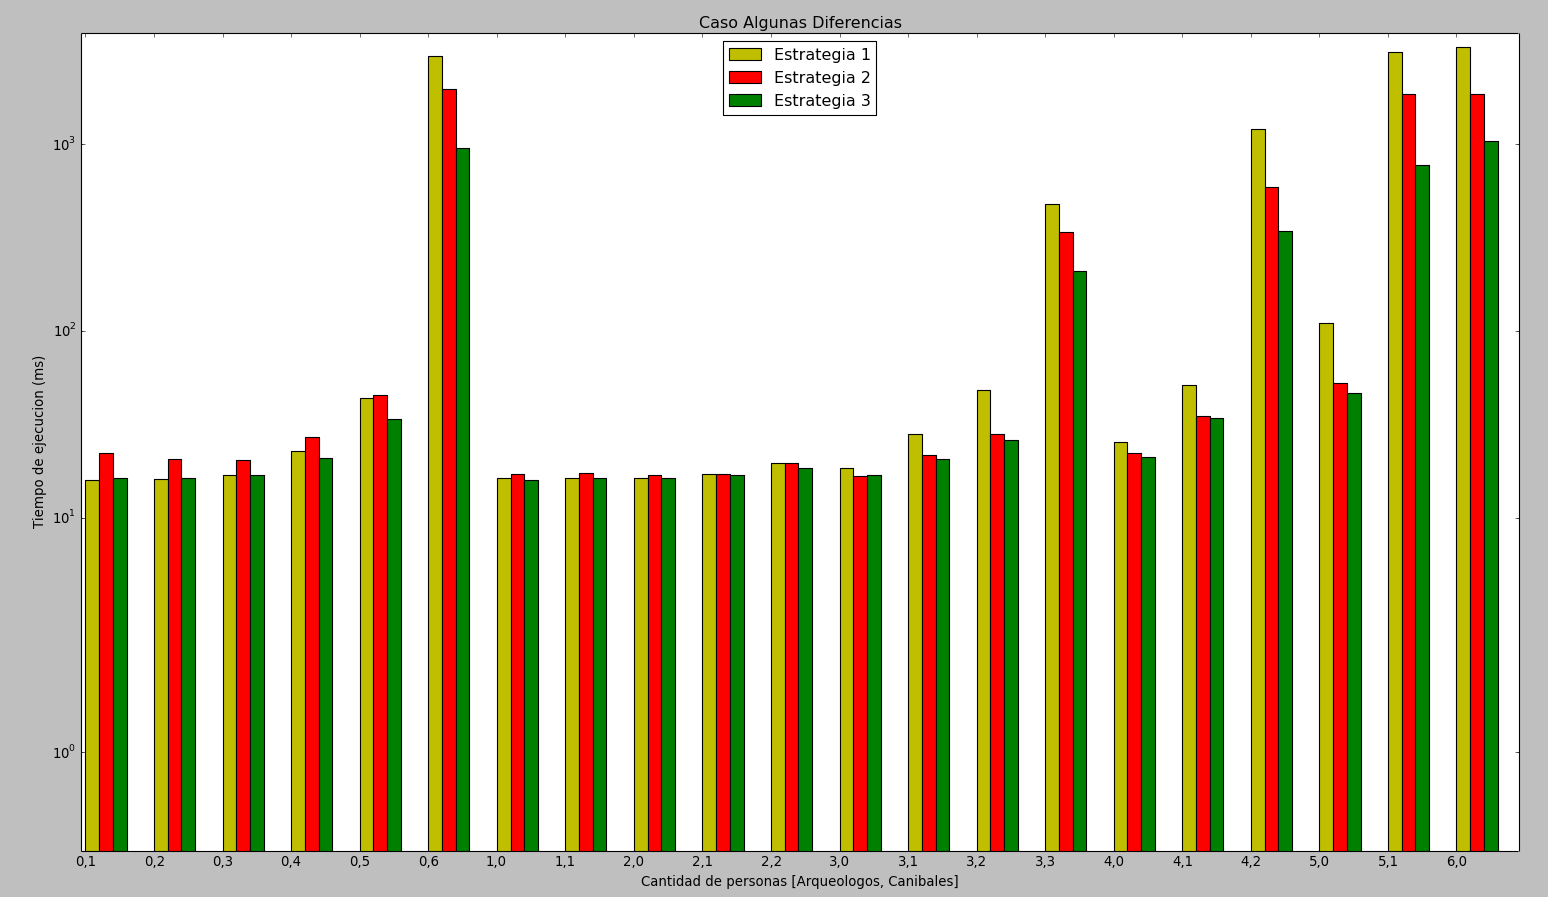
\includegraphics[width=1\textwidth,natwidth=610,natheight=642]{images/algunas_diferencias.png}
 \caption{Caso donde una mitad es diferente a la otra mitad.}
\end {center}
 \end{figure}
 %\begin {figure} [H]
%\begin {center}
 %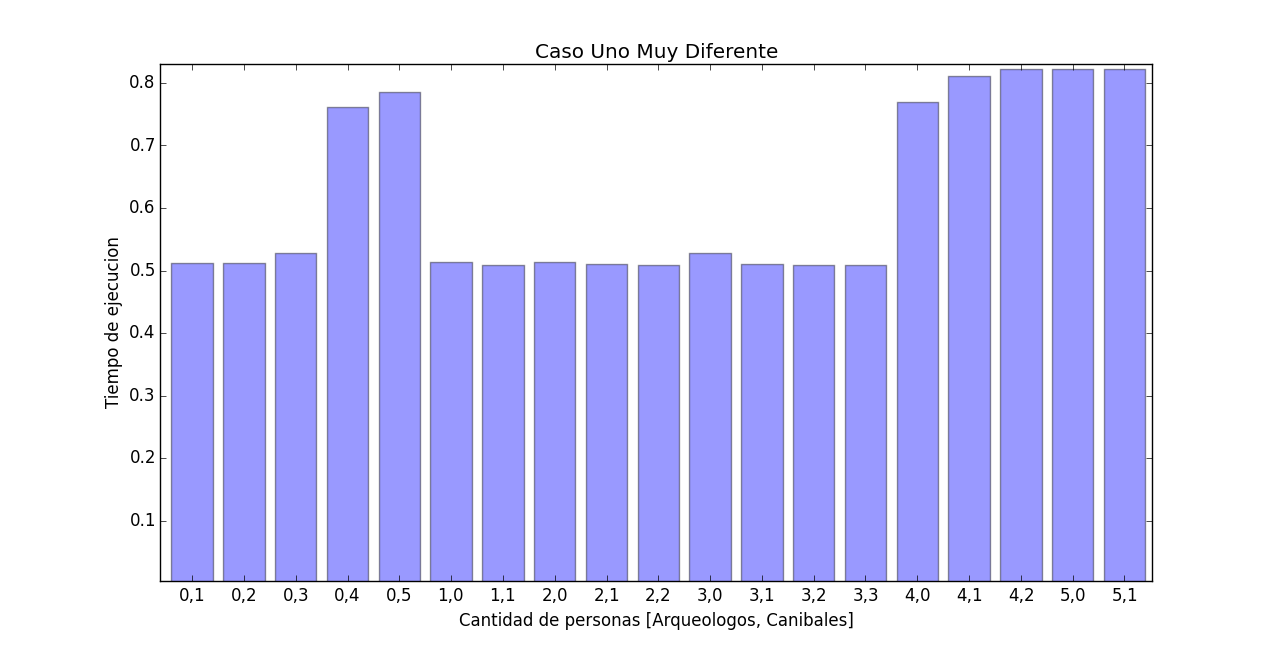
\includegraphics[width=1\textwidth,natwidth=610,natheight=642]{images/ej1_uno_muy_diferente.png}
 %\caption{Caso Uno Muy Diferente.}
%\end {center}
 %\end{figure}
 
%\begin{figure}
%	\centering
%	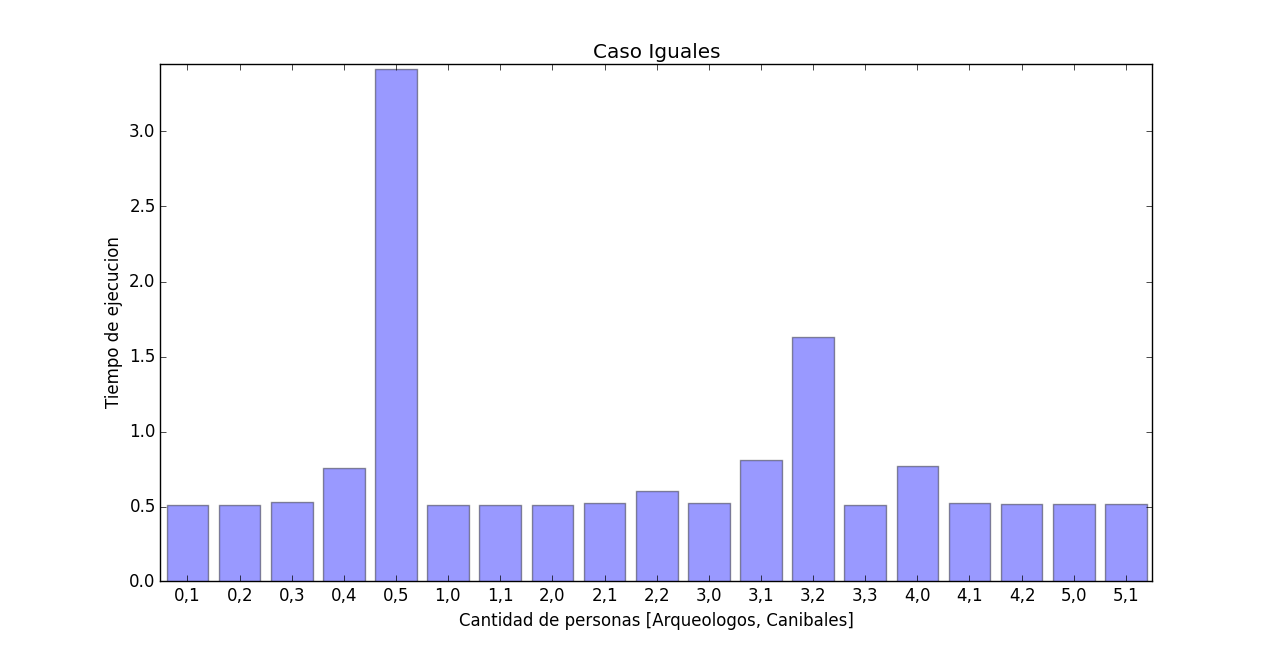
\includegraphics[width=1\textwidth]{images/ej1_iguales.png}
%	\caption{Caso Iguales}
%	\label{fig:ej1_iguales}
%\end{figure}
%\begin{figure}
%	\centering
%	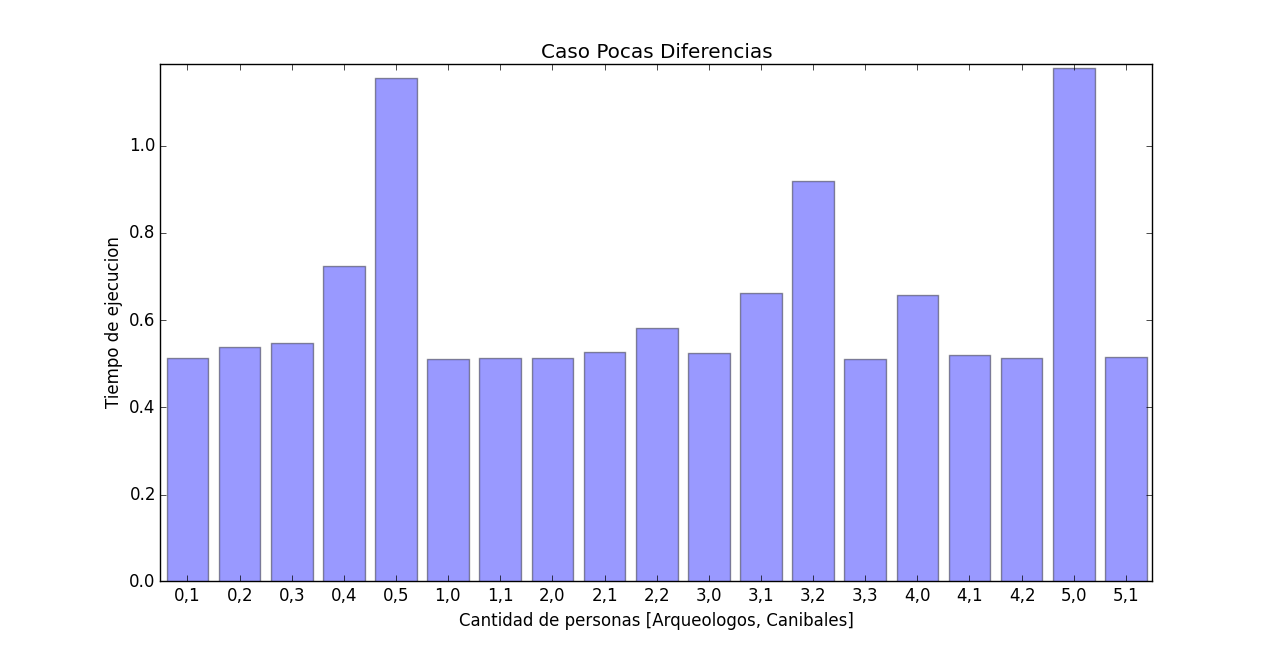
\includegraphics[width=1\textwidth]{images/ej1_pocas_diferencias.png}
%	\caption{Caso Pocas Diferencias}
%	\label{fig:ej1_pocas_diferencias}
%\end{figure}
%\begin{figure}
%	\centering
%	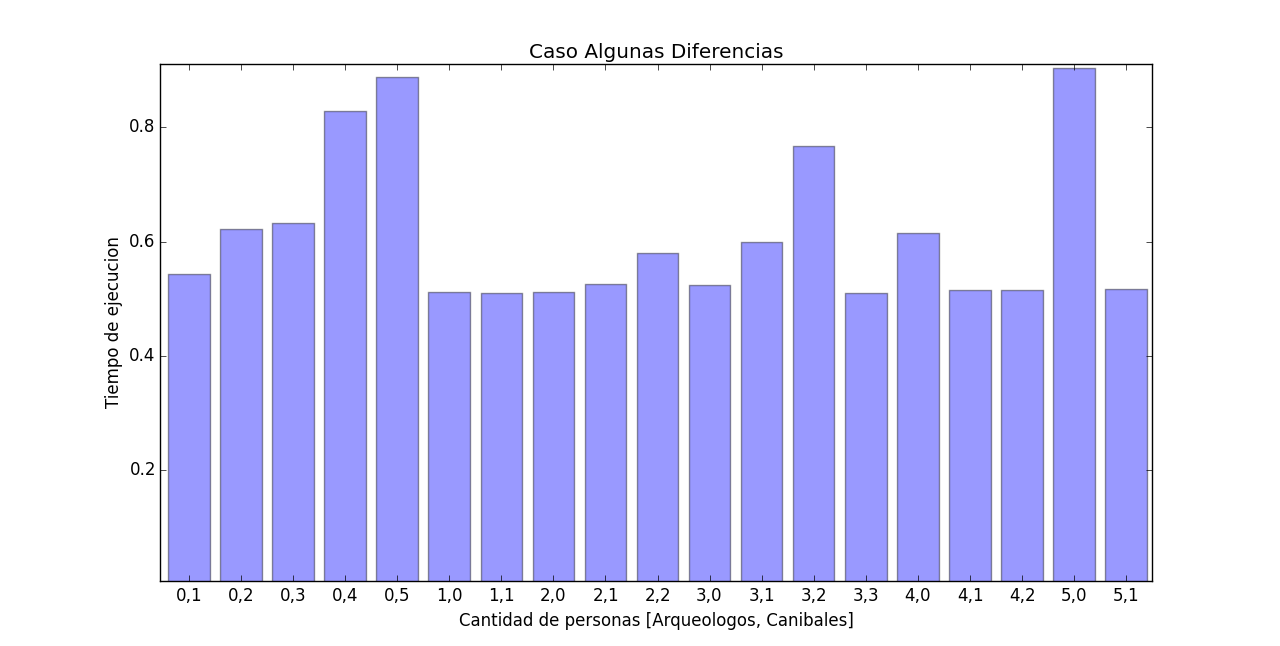
\includegraphics[width=1\textwidth]{images/ej1_algunas_diferencias.png}
%	\caption{Caso Algunas Diferencias}
%	\label{fig:ej1_algunas_diferencias}
%\end{figure}
%\begin{figure}
%	\centering
%	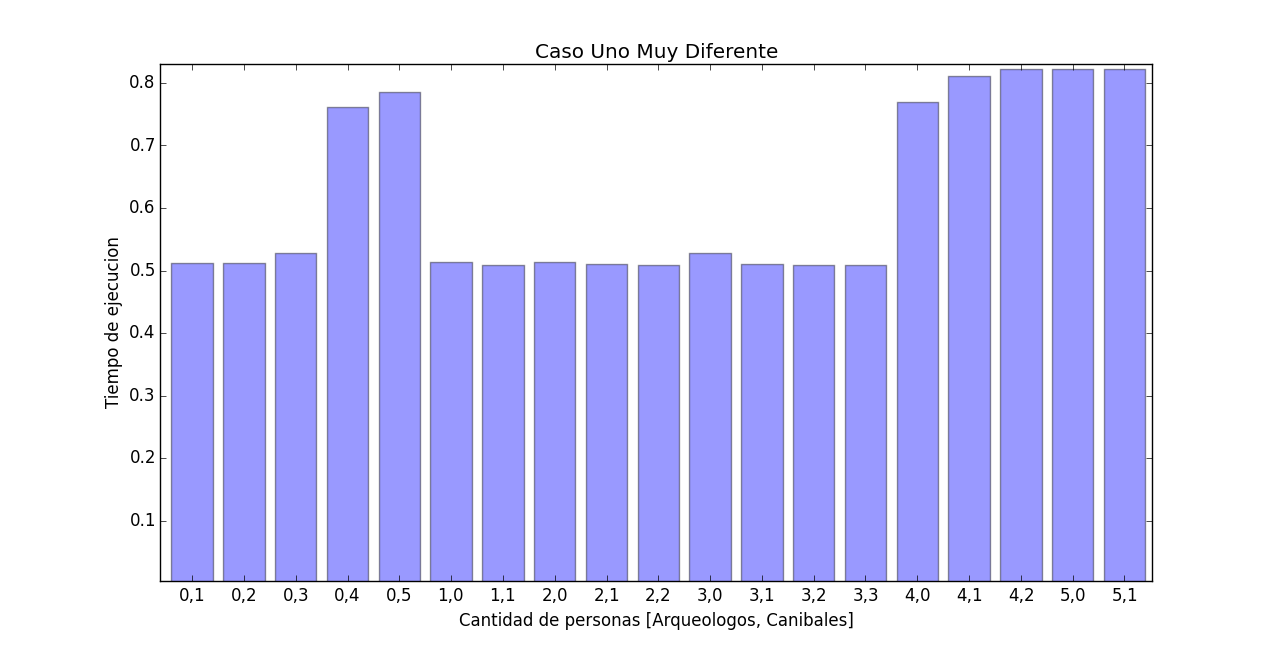
\includegraphics[width=1\textwidth]{images/ej1_uno_muy_diferente.png}
%	\caption{Caso Uno Muy Diferente}
%	\label{fig:ej1_uno_muy_diferente}
%\end{figure}


\par En los primeros tres gráficos  están plasmados los tiempos de ejecución de las distintas combinaciones de personas posibles en cada uno de los 3 casos mencionados previamente. 

\par Algo que podemos notar en el gráfico es que los picos mas altos se dan en combinaciones de personas con un tipo de persona (canibal o arqueólogo) igual a cero ó en casos de muchas personas. El resto de los casos se mantienen en un número similar. Vamos a ver estos dos casos que nombramos:

\begin{itemize}
	\item Caso con un valor igual a cero: \\
	Para este caso hay que remitirse a la condición mas importante que se debe respetar: \textit{No puede haber en ningún momento más personas del tipo canibal que del tipo arqueólogo en un mismo lado del puente}. Esta condición es muy relevante para este caso, ya que al ser la cantidad de uno de los dos tipos de personas igual a cero (no hay caníbales o no hay arqueólogos) entonces esta condición siempre se cumple. Lo cual nos lleva a que no hay casos que se puedan evitar (podar), se deben tomar todas las variantes posibles. Esto hace que su tiempo de ejecución se amplie notablemente.
	Podemos ver en los gráficos, que en los valores \textit{0,1}, \textit{0,2} y \textit{0,3} van en aumento, mientras que los valores \textit{0,5} y en \textit{0,6} ya son notáblemente grandes.
Es en estos casos donde notamos que la cota de complejidad depende en gran parte de la cantidad de personas, ya que todas las instancias son válidas y una rama no se va a cortar porque los caníbales se hayan comido a los arqueólogos.

	\item Caso con cantidad de personas cercana a 6: \\
	Observando los resultados se nota que otro pico en los tiempos de ejecución se da en la combinación `3 arqueólogos y 3 caníbales'. Este caso es particular porque la resolución del problema requiere que en un momento vuelvan dos personas, en vez de una como pasa generalmente. 
Casos como el de '$k$ arqs y $1$ caníbal' son similares a '$k+1$ arqs y $0$ caníbales', ya que en todos los casos tenemos la misma cantidad total de personas y todas las instancias son válidas (un sólo caníbal no puede invalidar una instancia.

\item Estrategias: En los casos que requieren mas tiempo computacional se ve como la estrategia $1$ le gana a la $0$. En la mayoría de las soluciones viaja una sola persona desde la derecha hacia la izquierda, salvo en el caso de 3 y 3 en el que un momento vuelven dos. La estrategia $1$ siempre prueba primero las soluciones donde viaja una persona de derecha a izquierda. Mientras que la estrategia $0$ empieza mandando de a dos, consiguiendo así todas soluciones sub-óptimas al principio. Entonces era esperable que la estrategia $1$ le gana a la $0$.
\\
La estrategia $2$ manda en un orden similar que la $1$, es decir, siempre comienza mandando de a dos de izquierda a derecha, y volviendo de a uno de derecha a izquierda. Con la salvedad de que cada vez que le toca mandar una persona de un lado a otro, siempre elije la mas rápida (primero del tipo caníbal y luego del tipo arqueólogo). Como explicamos en una sección anterior, esta estrategia consigue soluciones mejores mas rapidamente. 
En el gráfico se aprecia claramente como en todos los casos la estrategia $2$ es igual o mejor que la $1$, que ya de por sí era mejor que la $0$.  En los casos donde la complejidad es mayor se ve como la estrategia $2$ es bastante mejor que la $0$.
\end{itemize}

